\chapter{The Stakeholders}
\begin{figure}[ht]
  \centering
  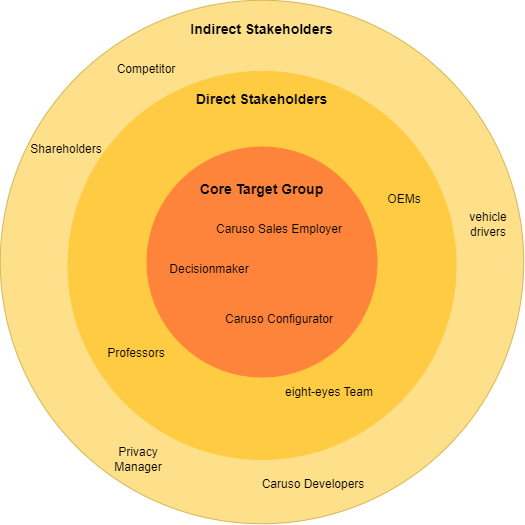
\includegraphics[width=12cm]{stakeholders/stakeholders.png}
  \caption{Stakeholders}
  \label{Kap2:Stakeholders}
\end{figure}
Die Abbildung \ref{Kap2:Stakeholders} zeigt die Stakeholder, die in Verbindung zu dem Projekt stehen. Die Stakeholder sind drei Kategorien unterteilt. Die Core Target Group sind die Stakeholder die das Produkt hauptsächlich Nutzen und somit nicht nur in direktem Kontakt mit dem Produkt stehen, sondern dieses auch nach Projektabschluss nutzen werden. Die direkten Stakeholder sind Personen oder Organistationen die mit dem Projekt in Kontakt stehen. Entweder arbeiten sind sie Mitarbeiter im Projekt, oder sie stellen Informationen bereit, die unabdingbar für das Projekt sind. Die indirekten Stakeholder sind alle Personen oder Organistationen, welche von dem erfolgreichen Projektabschluss profitieren, aber nicht mit dem Produkt in Verbindung stehen.
\section{Core Target Group}
Zur Core Target Group gehören die Cauros-Sales Mitarbeiter, die Entscheidungsträger der Kunden von Caruso sowie der Caruso Konfigurator. Im folgenden werden die Tätigkeiten der einzelnen Stakeholder erläutert und erklärt, warum diese wichtig für das abschließen des Projekts sind.

\subsection{Sales Mitarbeiter}
Die Caruso Sales Mitarbeiter sind die Personen, die Verträge mit den Entscheidungsträgern abschließen und somit die Schnittstelle von Caurso verkaufen. Zu ihren Tätigkeiten gehört:
\begin{itemize}
  \item Das Akquirieren neuer Kunden.
  \item Das Vorbereiten eines initialen Sales-Pitches beim Entscheidungsträger
  \item Das Präsentieren des Sales-Pitches mit dem Hintergrund das Vertrauen der Entscheidungsträger in die Daten zu erhalten.
  \item Das Klären von Fragen beim Kunden.
  \item Das Vorbereiten kundenbezogener Fahrzeugdaten.
  \item Das Abschließen des Vertrags mit den Entscheidungsträgern
\end{itemize}
Die Caruso Sales Mitarbeiter sind an dem aktuellen und zukünftigen Workflow für das Akquirieren neuer Kunden unabdingbar und waren die Hauptansprechpartner während der Design Sprints.

\subsection{Decisionmaker}
Die Entscheidungsträger sind die Kunden Caursos, welche Interesse an den zur Verfügung gestellten Daten haben. Diese Entscheidungsträger sind bei mittelständischen Unternehmen größtenteils die Inhaber der Firma, welche mit den Daten von Caruso neue Anwendungen entwicklen wollen, um den Worklflow in ihrere eigenen Firma zu verbessern. Nach Aussagen von Caruso sind die rentabelsten Entscheidungsträger Versicherungen, Pannenhilfen oder Werkstätte. Während des Design Sprints war es nicht möglich Kontakt zu diesen Stakeholdern aufzunehmen, jedoch sind ihre Interessen unabdingbar, um ein Produkt zu entwerfen, was sie davon überzeugt in die Caurso-Schnittstelle zu investieren. Ihre Interessen wurden über die Sales Mitarbeiter von Caruso erhoben, welche stellvertretend ihre Interessen bewarben.
\begin{itemize}
  \item Sie entscheiden über den Vertragsabschluss mit Caruso für ihre Firma.
  \item Sie haben wenig technische Kentniss.
  \item Sie kaufen nur etwas, in das sie einen Mehrwert sehen.
\end{itemize}

\subsection{Configurator}
Die Cauros Konfiguratoren sind die Mitarbeiter, welche die Daten der Kunden sammeln und über einen Excel oder HTML-Bericht zusammenfassen. Sie sind technische Mitarbeiter, die auf Anfrage der Sales-Mitarbeiter die Daten für die Sales-Pitches bereitstellen. Zu ihren Aufgaben gehört
\begin{itemize}
  \item das Sammeln der Fahrzeugdaten
  \item das Erstellen der Excel oder HTML-Berichte.
  \item das Anpassen der Berichte an kundenspezifische Wünsche.
\end{itemize}
Im Idealfall werden die Konfiguratoren nach diesem erfolgreichen Projektabschluss nicht mehr benötigt, da die Anwendung automatisch Fahrzeugdaten sammelt und von den Sales Mitarbeitern konfiguriert wird.

\section{Other Stakeholders}
Zu den anderen Stakeholdern gehören die direkten und indirekten Stakeholder. Diese werden im weiteren Verlauf des Projekts nicht betrachtet, weil sie das Ergebnis des Produkts nicht beeinflussen. Im folgenden werden zu den Stakeholdern eine Kurzbeschreibung gegeben.

\subsection{Direkte Stakeholder}
\begin{itemize}
  \item eight eyes Team: Das eight eyes Team hat die Anforderungen an das System erhoben und bietet den nachfolgenden Entwicklern die Grundlage zur Entwicklung der Anwendung.
  \item Professoren: Die Professoren stellen den intialien Kontakt zum Kunden bereit und organisieren die zentralen Ereignisse für das Projekt.
  \item OEMs: Die OEMs stellen die Fahrzeuginformationen zur Verfügung, welche von Caruso überhaupt standardisiert werden können. Ohne diese Daten könnte die Anwendung gar nicht entwickelt werden.
\end{itemize}
\subsection{indirekte Stakeholder}
\begin{itemize}
  \item Stakeholder: Die Shareholder investieren in das Unternehmen Caruso und profitieren somit von weiteren Vertragsabschlüssen von Caruso, wenn sie durch dieses Projekt mehr Kunden akquirieren können.
  \item Konkurrenz: Diese Firmen werden negativ von dem Erfolg von Caruso beeinflusst.
  \item Autofahrer: Die Autofahrer sind die Kunden der Entscheidungsträger. Sie profitieren, wenn beispielsweise eine Werkstatt einen besseren Kundenservice anbieten kann, indem sie die Caruso-Plattform nutzen.
  \item Die Caruso-Entwickler: Die Entwickler werden in der Zukunft das zu entwickelnde System erweitern.
  \item Datensicherheitsbeauftragter: Diese Personen handhaben die Datensicherheit für Caruso. In der Praxis achtet Caruso auf den Datenschutz ihrerer Kunden, jedoch sollen nach Aussage von Caruso für dieses Projekt Datenschutzbedenken vernachlässigt werden.
\end{itemize}

\section{Personas}
\begin{itemize}
  \item Rüdiger Rübe (Entscheidungsträger)
  \item Cornelius (Sales)
  \item Konfigurator?
\end{itemize}